\subsection{Inbetriebnahme}
\label{subsec:inbetriebnahme}

In diesem Kapitel wird die erste Inbetriebnahme des Roboters beschrieben.
Hierzu werden auch die Inhalte und Erweiterungen aufgelistet, welche im Lieferumfang für einen \gls{go1} Edu enthalten sind.
Anschließend soll der Betrieb durch den Akku und ein Netzteil beschrieben werden.

% todo an aus fernbedienung?

\subsubsection{Lieferumfang}

Abbildung \ref{fig:lieferumfang} zeigt die im Lieferumfang enthaltene Transportbox aus Styropor und deren Inhalte, welche
gleichzeitig der gesamte Lieferumfang des \gls{go1} in der \emph{Edu} Version ist.

\begin{figure}[h]
    \frame{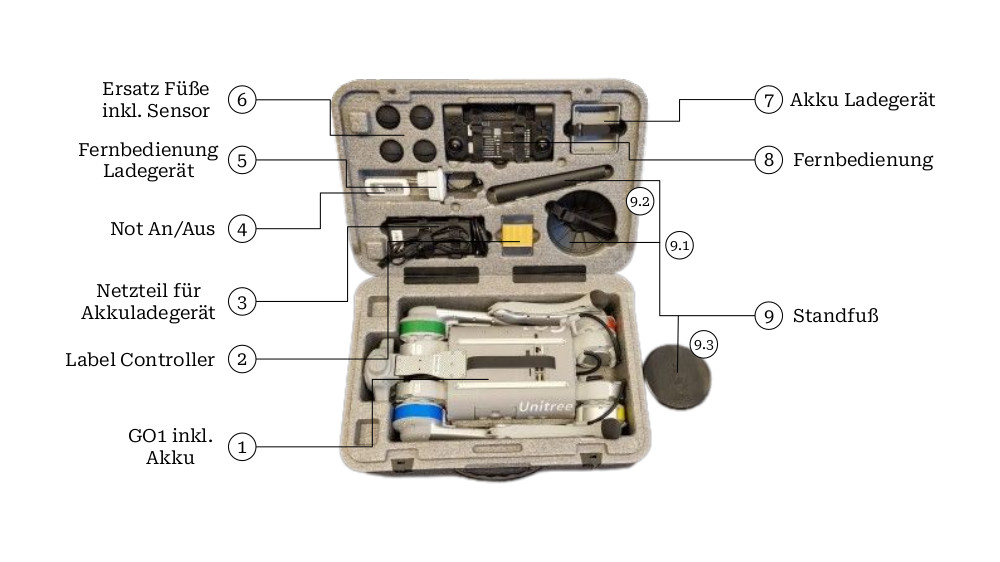
\includegraphics[width=\linewidth]{img/analyse/lieferumfang}}
    \caption{Ansicht der Transportbox und des Lieferumfangs}\label{fig:lieferumfang}
\end{figure}

\noindent Im Lieferumfang enthalten sind folgende Elemente:

\begin{enumerate}
    \item \gls{go1} inklusive Akku
    \item Kompakte Fernbedienung mit \emph{Folge-Mir}-Funktion
    \item Netzteil für das Akku-Ladegerät
    \item Fernbedienung für An-/Ausschaltfunktion
    \item Ladegerät für die Fernbedienungen inklusive \gls{usb}-A auf \gls{usb}-C Kabel
    \item Vier Ersatzfüße inklusive der integrierten Drucksensoren
    \item Akku-Ladegerät mit \gls{usb}-C Anschluss zur Akkuinspektion
    \item Fernbedienung
    \item Standfuß aus drei Teilen für die Ablage des \gls{go1}
    \begin{enumerate}
        \item Sockel
        \item Verlängerung
        \item Plattform inklusive Einkerbungen zum Ausbalancieren des aufliegenden \gls{go1}
    \end{enumerate}
\end{enumerate}

Sollte kein weiteres Zubehör konfiguriert sein, so sind an den Montagestellen auf der Oberseite des Roboters Gummienden
zum Schutz des Korpus bei Rotationen montiert.
Je nach bestelltem Zubehör - wie beispielsweise eines professionellen \gls{lidar} Sensors oder eines
Roboterarmes am \gls{go1} - sind Schienen an der Oberseite des Rumpfes montiert.
In diesem Fall werden die Gummienden sowie eine Schutzabdeckung für die Entwicklerports, die standardmäßig montiert ist,
in der Transportbox mitgeliefert.

\subsubsection{Mobile Inbetriebnahme}
\label{subsubsec:inbetriebnahme_akku}

Als mobile Inbetriebnahme wird hier die Inbetriebnahme des Roboters mit einer Stromversorgung durch den Akku bezeichnet.
Für die Inbetriebnahme auf diese Weise sind folgende Teile nötig:

\begin{requirements}
    \gls{go1}, Akku, Akkuladegerät inklusive Netzteil, Fernbedienung inklusive Ladegerät
\end{requirements}

\noindent Zur Vorbereitung müssen sowohl Akku als auch die Fernbedienung geladen werden.
Sind diese ausreichend geladen, kann der Akku eingesteckt und der \gls{go1} in die Ausgangsposition gebracht werden.
Hierfür müssen die vier Beine so rotiert werden, dass sowohl Fuß als auch Knie den Boden berühren.
Abbildung \ref{fig:ausgangsposition} zeigt die Ausgangsposition des Roboters.

\begin{figure}[h]
    \frame{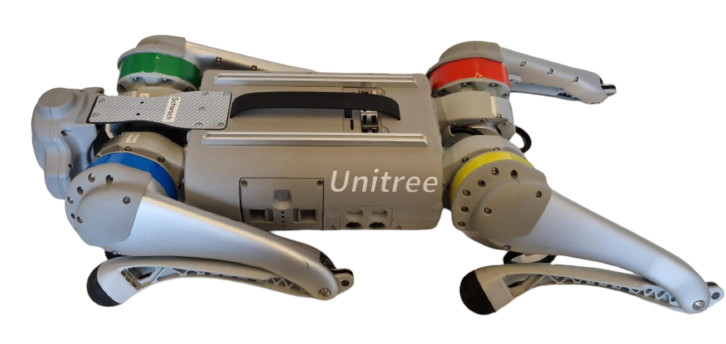
\includegraphics[width=\linewidth]{img/analyse/ausgangsposition}}
    \caption{Ausgangsposition des Roboters}\label{fig:ausgangsposition}
\end{figure}

Durch einfaches Drücken auf dem Knopf neben der Ladeanzeige des Akkus wir der Ladestand über die vier \glspl{led}
angezeigt.
Durch ein sofortiges weiteres Drücken und Halten des Knopfes startet der Roboter.
Dies wird über ein kurzes serielles Aufblinken aller vier \glspl{led} signalisiert.
Zudem sind die Lüfter deutlich zu hören.
Durch dasselbe Verfahren - Drücken gefolgt von zweitem Drücken und Halten des Knopfes neben der Ladeanzeige auf
der Unterseite der Fernbedienung wird auch diese angeschaltet.
Ein einmaliges akustisches Signal ertönt beim Anschalten.
Die Fernbedienung verbindet sich automatisch mit dem Roboter.
Im Werkszustand steht der Roboter nach dem Einschalten nach etwa \num{70} - \num{80} Sekunden auf.
Der Roboter kann nun über die Fernbedienung gesteuert werden.

Zum Ausschalten des \gls{go1} sollte dieser in eine liegende Position (\emph{Prone}-State) und anschließend in den \emph{Damping}-State gebracht werden.
Das wird durch die Tastenkombinationen \texttt{L2+A} und \texttt{L2+B} erreicht.
Danach kann der Akku wie beim Anschalten durch Drücken und erneutes Drücken und Halten ausgeschalten werden.
Die \glspl{led} signalisieren das erfolgreiche Ausschalten und die Lüfter schalten sich aus.
Auch die Fernbedienung kann durch dieses Vorgehen ausgeschalten werden.
Hier signalisieren drei kurze akustische Signale das erfolgreiche Ausschalten.

\subsubsection{Stationäre Inbetriebnahme}
\label{subsubsec:inbetriebnahme_netzteil}

Im Gegensatz zur mobilen Inbetriebnahme wird hier die Inbetriebnahme des Roboters durch eine stetige Stromversorgung durch ein Netzteil
bezeichnet.
Hierfür müssen einige Vorbereitungen getroffen werden, da im Lieferumfang kein Netzteil für den Betrieb des \gls{go1}
enthalten ist.

\begin{requirements}
    \gls{go1}, Netzteil für Akkuladegerät\newline
    \textbf{Zusätzlich:} Hohlstecker M \num{5,5}/\num{2,1} mm auf Schraubklemme, XT30-M Stecker mit ausreichend (> \num{10} cm)
    Verkabelung.
    Alternativ: XT30-M auf Hohlstecker M \num{5,5}/\num{2,1} mm Adapter.
\end{requirements}

Vergleicht man Ausgangsspannung und maximale Stromstärke des verbauten Akkus mit den selben Werten des Netzteils für das
Akkuladegerät, so erkennt man, dass das Ladegerät die passende Ausgangsspannung und Leistung vorweist, um den \gls{go1}
über den in Kapitel \ref{subsubsec:recheneinheiten} Abbildung \ref{fig:vogelperspektive} beschriebenen \emph{XT-30} Port
zu betreiben.
Da das Netzteil lediglich einen Hohlstecker zum Anschluss bietet, muss hierfür jedoch in Eigenarbeit ein Adapter auf XT-30
hergestellt werden.
Herbei sind die in den Ressourcen beschriebenen Bauteile nötig, die Schraubverbindung ist zwar optional und kann durch eine
Lötstelle oder ein vorgefertigtes Teil ersetzt werden, sie erleichtert jedoch die Beschaffung und den Zusammenbau des Adapters.
Zu beachten ist hierbei nur ide korrekte Abmantelung der Kabel für die Schraubklemme und die Orientierung der Kabel in der
Klemme.
Abbildung \ref{fig:xt30} zeigt eine beispielhafte Umsetzung des Beschriebenen und die korrekte Orientierung des XT-30 Steckers.

\begin{figure}[h]
    \frame{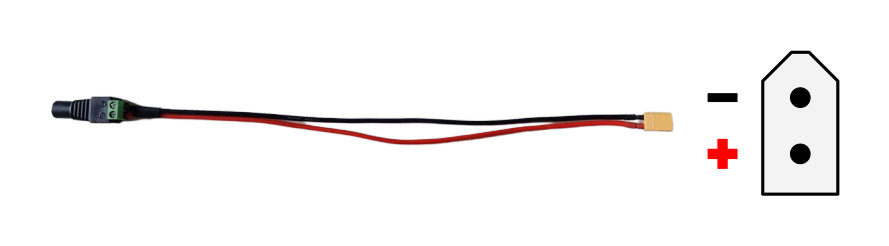
\includegraphics[width=\linewidth]{img/analyse/xt30}}
    \caption{XT-30 auf Hohlstecker Verkabelung und XT-30 Orientierung}\label{fig:xt30}
\end{figure}

Aus Sicherheitsgründen sollte der sogenannte \emph{Sportmodus} des \gls{go1} deaktiviert werden, da sich dieser sonst nach
Start des Roboters aufsteht, was die Verkabelung lösen könnte.
Zudem ist die maximale Ausgangsleistung des Netzteils nicht hoch genug, um den Roboter dauerhaft inklusive der Motoren
zu betreiben.
Der Betrieb wird deshalb stationär genannt.
Für das Deaktivieren des Sportmodus muss sich zunächst auf den Raspberry Pi verbunden werden.
Im Home-Ordner des Nutzers \emph{pi} befindet sich der Ordner \texttt{Unitree/autostart/triggerSport} mit der Datei
\texttt{trig\-ger\-Sport.sh}.
Diese muss lediglich umbenannt werden, beispielsweise zu \texttt{trig\-ger\-Sport.dis\-a\-bled.sh}.

\begin{lstlisting}[language=sh,label=lst:disable-triggersport]
pi@raspberrypi:~ $ cd Unitree/autostart/triggerSport/
pi@raspberrypi:~/Unitree/autostart/triggerSport $ ls
build  log  triggerSport.sh  version.txt
pi@raspberrypi:~/Unitree/autostart/triggerSport $ mv triggerSport.sh triggerSport.disabled.sh
pi@raspberrypi:~/Unitree/autostart/triggerSport $ ls
build  log  triggerSport.disabled.sh  version.txt
\end{lstlisting}

\noindent Beim Neustart des Roboters wird nun nicht automatisch in den Sportmodus geschaltet und die Motoren bewegen sich nicht.
Weiteres zur \emph{Autostart}-Funktion des \gls{go1} in Kapitel \ref{subsubsec:software-autostart}.

Zuletzt kann das Netzteil inklusive des Adapters in den XT-30 Port auf dem Rücken des Roboters gesteckt werden.
Ein erfolgreicher Start des Roboters kann über das akustische Wahrnehmen der Lüfter geprüft werden.
Zum Ausschalten muss der Stecker lediglich entfernt und der Roboter somit vom Strom getrennt werden.
Hierfür muss nur sichergestellt sein, dass alle manuellen Operationen auf den Recheneinheiten vollendet sind, damit diese
nicht korrumpiert werden.

\subsubsection{Anwendungen}
\label{subsubsec:anwendungen}

Nach Inbetriebnahme des \gls{go1} stehen dem Nutzer zwei grafische Anwendungen zur Verfügung, mit denen er Funktionen
des Roboters wie Monitoring, Steuerung und Simulationen ausführen kann.
Dieses Kapitel soll kurz die erste Einrichtung beziehungsweise Öffnen der Anwendungen dokumentieren.

\myparagraph{Webinterface}

Der Raspberry Pi des \gls{go1} startet zum Systemstart automatisch einen Webserver mit einer Webseite, die diverse Funktionen
zugänglich macht.
Für das Aufrufen der Webseite muss man sich im selben Netzwerk wie der \gls{go1} befinden.
Weitere Informationen hierzu sind in den Kapiteln \ref{subsubsec:lokales-netzwerk} und \ref{subsubsec:netzwerk} beschrieben.
Auf dem \gls{http}-Port \num{80} des Pis\footnote{Erreichbar auf \texttt{192.168.123.161} oder \texttt{192.168.12.1} im eigenen WLAN-Hotspot (Siehe \ref{subsubsec:lokales-netzwerk})}
ist nun die Seite aufrufbar.
In Browsern reicht hierfür lediglich die Eingabe der \gls{ip} Adresse, der Port muss nicht definiert sein.
Abbildung \ref{fig:website} zeigt eine Bildschirmaufnahme des Webinterfaces.

\begin{figure}[h]
    \frame{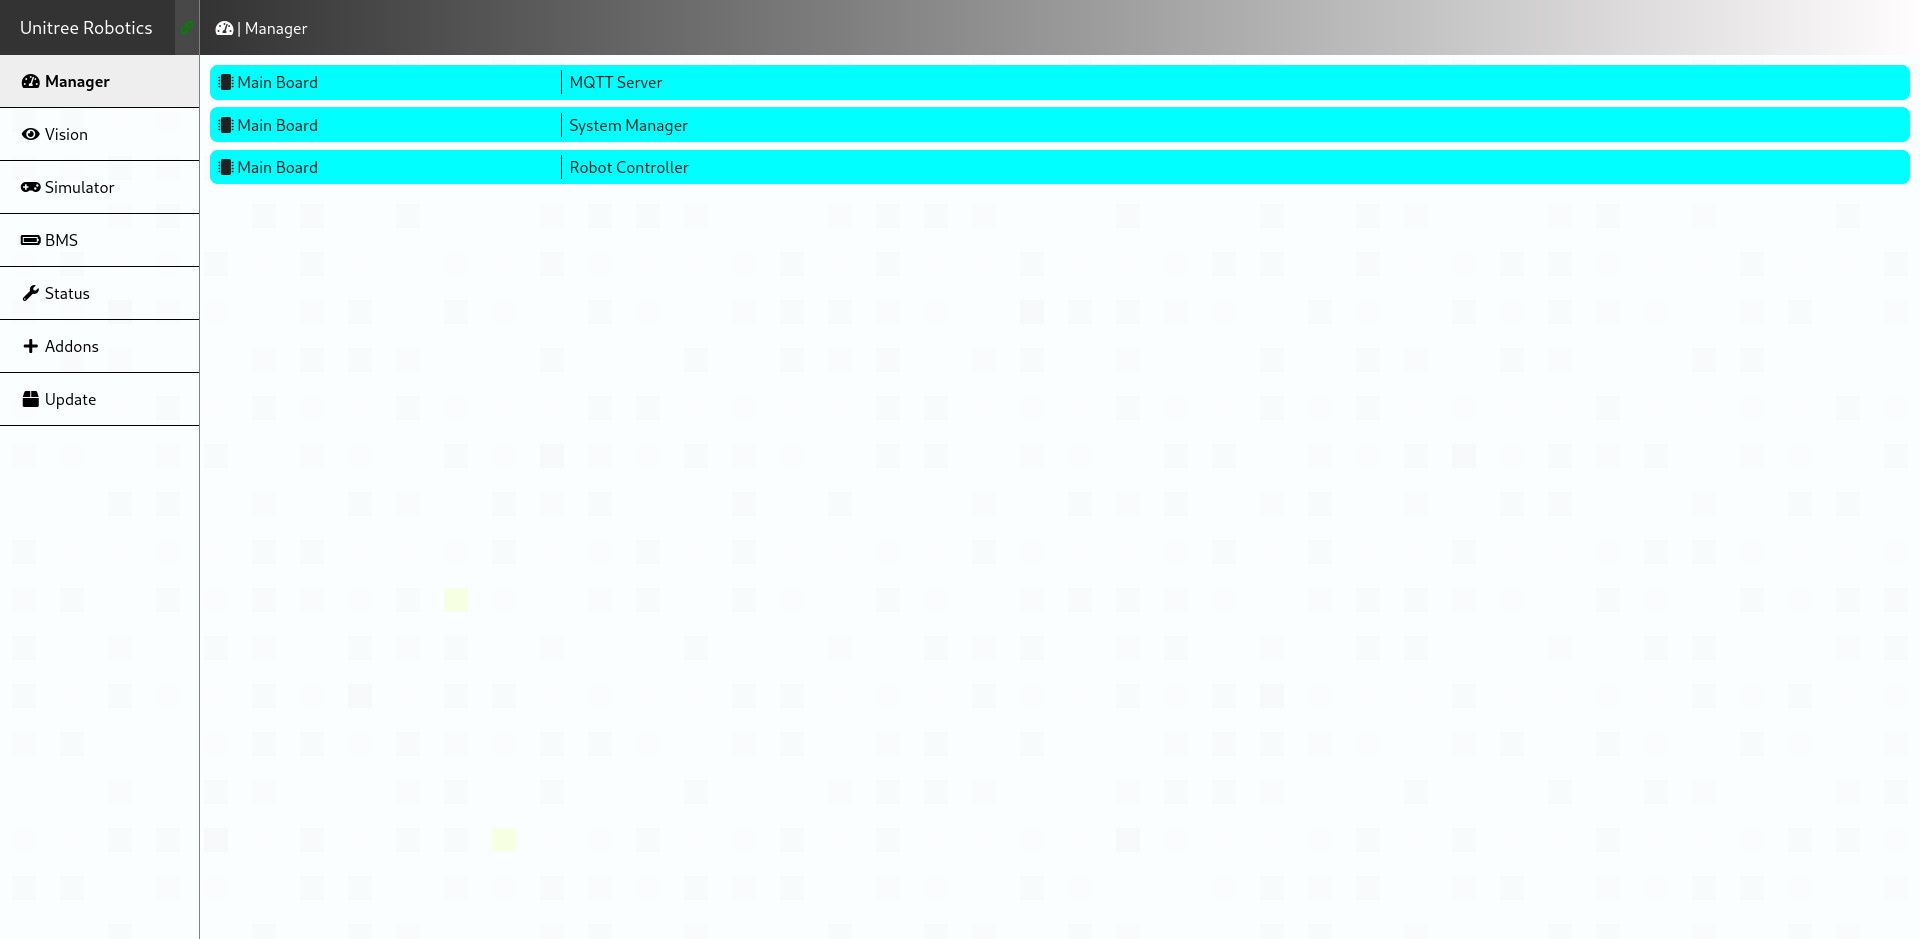
\includegraphics[width=\linewidth]{img/analyse/website}}
    \caption{Screenshot des Webinterfaces}\label{fig:website}
\end{figure}

\myparagraph{Mobile App}

Unitree Robotics hat als Ergänzung zum Webinterface ebenfalls eine mobile Anwendung für die Plattformen \emph{iOS} und
\emph{Android} veröffentlicht.
Diese kann fertig gebaut von der Entwicklerwebseite heruntergeladen werden und muss auf den jeweiligen Plattformen als
fertige App aus unbekannter Quelle installiert werden\footcite{unitree_app_download}.
Hierfür sind in der Regel die Entwickleroptionen zu aktivieren.
Da die Installationsprozesse für die Plattformen und Endgeräte unterschiedlich sein können, wird in dieser Arbeit nicht
darauf eingegangen.
\footnote{Weitere Informationen zur Installation von Beta-Apps für iOS auf \url{https://testflight.apple.com/join/KraKgqam}
und für Android auf \url{https://www.heise.de/tipps-tricks/Externe-Apps-APK-Dateien-bei-Android-installieren-so-klappt-s-3714330.html}}
Abbildung \ref{fig:android} zeigt zwei Bildschirmaufnahmen der mobilen Anwendung.

\begin{figure}[h]
    \frame{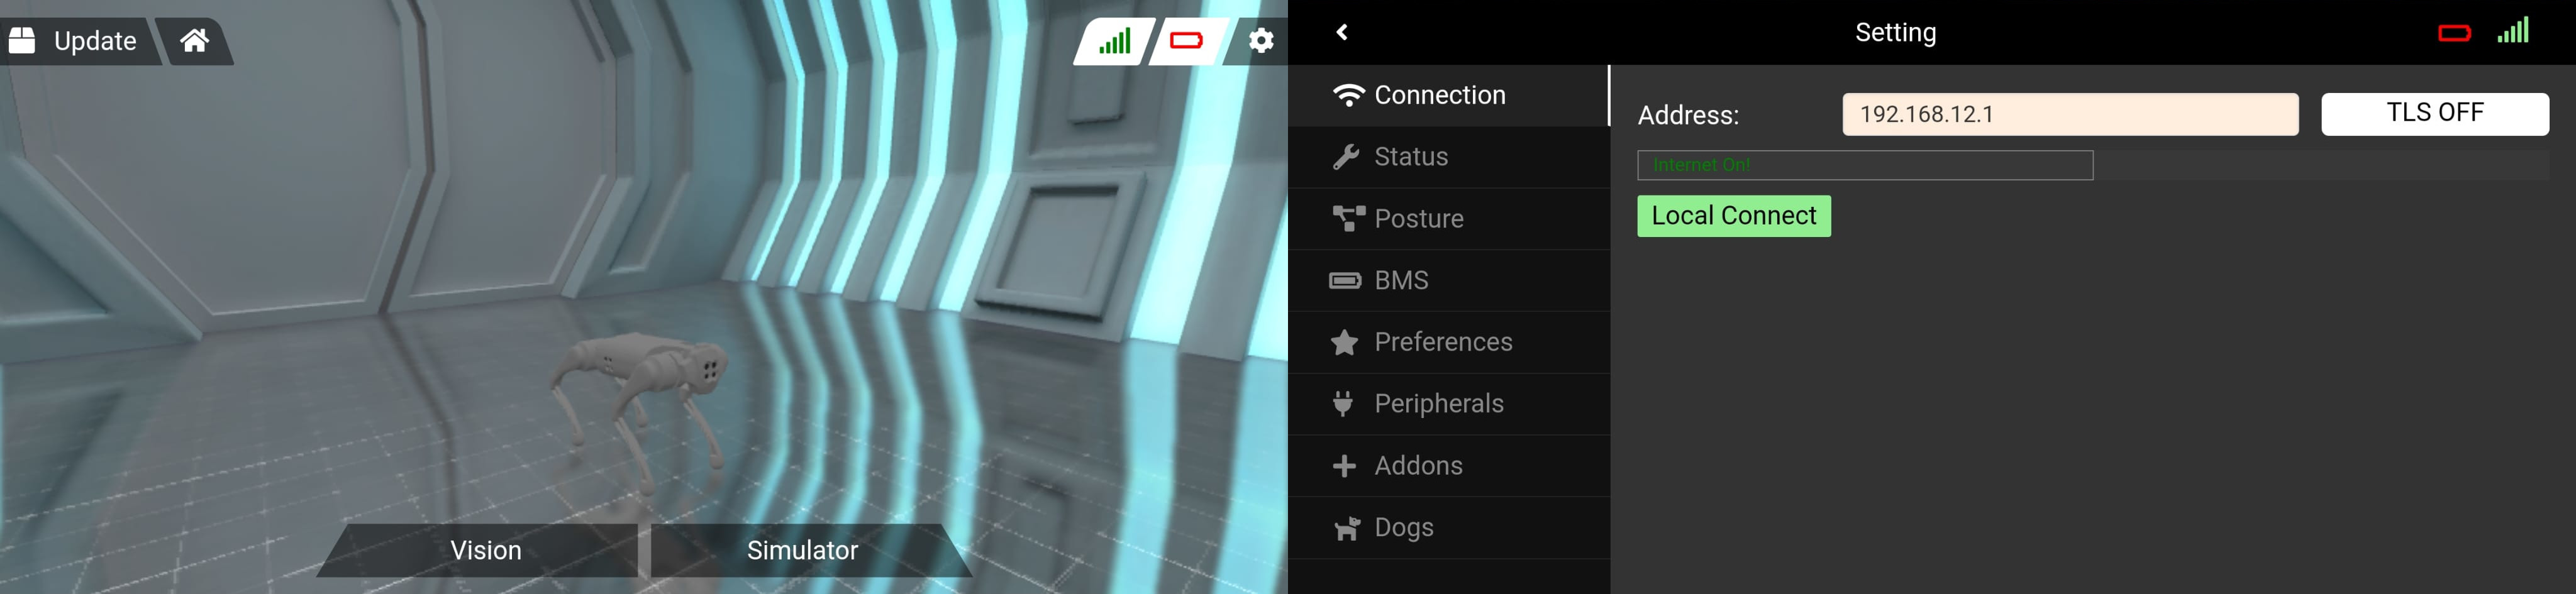
\includegraphics[width=\linewidth]{img/analyse/android}}
    \caption{Screenshot der mobilen Anwendung}\label{fig:android}
\end{figure}

\noindent Für die Verbindung zum Roboter muss sich lediglich mit dem Netzwerk des Roboters verbunden werden.
Die \gls{ip} Adresse des Roboters muss dann noch in den Einstellungen hinterlegt werden.
Danach können die Informationen vom \gls{go1} über die Anwendung eingesehen werden.